\documentclass{article}
\usepackage{hyperref}
\usepackage[margin=1in]{geometry}
\usepackage{indentfirst}   % Indents first paragraph. change if u want ig
\usepackage{setspace} 
\doublespacing
\usepackage{graphicx}
\graphicspath{ {images_arch} }
\usepackage{listings}
\usepackage{xcolor}
\lstset{
  basicstyle=\ttfamily,
  columns=fullflexible,
  breaklines=true,
  postbreak=\raisebox{0ex}[0ex][0ex]{\color{red}$\hookrightarrow$\space}
}

\begin{document}
\title{\textbf{Final Undergraduate Psuedo-Sudoku Submission}}
\author{Spencer Hirsch, Thomas Johnson}
\date{\today}

\maketitle

\noindent \textbf{Summary of Project}

\medskip

Following our original submission we have implemented another algorithm. With 
our original submission we implemented a backtracking algorithm, which worked
very well for our first milestone. For this final milestone we have implemented
a backtracking with a heuristic algorithm. Both algorithms solve the given
test cases, however after doing an analysis of the two comparing the input size and
the number of removed cells there is a clear difference in the complexity of the
two different algorithms. 

In order to generate reasonable test cases to demonstrate the time complexity of our
our two algorithms. We have implemented a generator to generate test cases to give to
our algorithms. Each algorithm tests a total of 2700 different test cases with varying
difficulty. The goal of implementing a generator was to make the tests as random as 
possible and to easily generate a larger sum of test cases. For each n (the size of 
the matrix, n x n) there are 15 additional test cases that have varying m (number of 
missing cells). Each of these n x m combinations is tested a total of 30 times. This 
is how we have determined that there are a total of 2700 different test cases run on
each of the algorithms. 

All aspects of the board aside from the size of the board is randomly determined. The 
values for each squares are randomly assigned for the size of the board. Once all of
the values are determined the number of removed cells is randomly selected and unique 
to each row. The purpose of creating this random algorithm was to ensure that bias was 
reduced. 

In order to demonstrate the time complexity of each of the algorithms the cpu time is
recorded for each test and plotted against the number of removed squares from the sudoku
board. To ensure the accuracy of our results the same test cases are run on both of the
algorithms. Two scatter plots are constructed for the two algorithms, one displaying every
point gathered from the test sets and the other plot demonstrating the averages of the 15
ponints for each n x m pair. 

\pagebreak

\noindent \textbf{Backtracking Algorithm}

\begin{lstlisting}[frame=single]
	# Find next empty cell in the matrix
	def find_cell(board, size): -> int, int
		for i in range size:
			for j in range size:
				if board[i][j] is empty
					return i,j 
		return -1, -1 # Full board, return sentinal values -1, -1

	# Function checks for a valid move given the value of the current cell
	def valid_move(cord1, cord2, board, size, number): -> boolean
		# Given current cordinatess iterate through the row, and column
		# to make sure psuedo sudoku rules are not violated
		for i in range size:
			if board[i][cord2] = number 
			return false
		for j in range size:
			if board[cord1][j] = number
			return false
		return true
	
	# Implements the full back tracking algorithm
	solve(board, size): -> boolean
		nums = list(1, ... N + 1)	# stores all possible numbers
		cord1, cord2 = find_cell (board, size) # finds the next position
		if cord1 and cord2 == -1: # board is filled with legal moves
			return true
		for num cell in nums	# iterates through every possible move
			if valid_move(cord1, cord2, board, size, num):
				board[cord1][cord2] = num
				if solve(board, size):	# continue down this branch
					return true
				board[cord1][cord2] = 0	# failure, begin back tracking
		return false # could not be solved
\end{lstlisting}

\textit{How the backtracking algorithm works:} \\

\medskip
	The original algorithm is built on the idea of back tracking. To begin we first
	need to have an array storing all possible number selections for an NxN board. This means that
	if the board is 3x3 we will store the numbers [1, 2, 3] in the array \verb|nums|. The next step is to find which cell we should
	make the next valid move in, using \verb|cord1, cord2 = find_cell(board, size)|. This function works simple enough;
	it merely iterates through the rows, and columns of the inputted board to find the next blank space. 
	If no empty space is found we return the values -1, -1. This signifies the board is filled up fully, and that it is solved.

	Moving into the main bulk of the algorithm, we enumerate through each \verb|num in nums|, and use the code
	\verb|if valid_move(cord1, cord2, board, size, num)|. \verb|valid_move(...)| works on taking in the required information,
	and seeing if the current \verb|num| is a valid move at that cordinate given the ruleset of psuedo sudoko. If it is valid we return true
	else we return false, and move on to another number. If its a valid move however we set that boards cell to the current number
	\verb|board[cord1][cord2] = num|.

	Now that a valid move has been found we begin to recursively call the function using the code \verb|if solve(board, size)|. If this evaluates to true
	then the board will recursively be filled up with valid moves. However if \verb|solve(...)| evaluates to false at any point in time, the current cell is reflagged 
	as empty, and the back tracking begins. \\



\pagebreak

\noindent \textbf{Backtracking with Heuristic}

\begin{lstlisting}[frame=single]
	# Functions used prior that are unchanged:
	def find_cell(board, size) -> int, int
	def valid_move (cord1, cord2, board, size, number) -> boolean

	# New function to implement basic forward checking
	def get_unused_numbers(board, cord1, cord2, size) -> list
		nums = set of the range(1, size + 1) to hold all possible values.

		# Iterate through the row, and column of current cords to remove duplicates
		for i in range of size:
			current number = board[i][cord2]
			if current number is in nums:
				remove current number from nums
		for j in range of size:
			current number = board[cord1][j]
			if current number is in nums:
				remove current number from nums
		return list(nums)

	# This will slightly the code for solve2
	def solve2 (board, size):
		cord1, cord2 = find_cell (board, size) -> int, int
		nums = get_unused_numbers(board, cord1, cord2, size) -> list
		if cord1 and cord2 == -1:
			return true
		for num cell in nums
			if valid_move(cord1, cord2, board, size, num):
				board[cord1][cord2] = num
				if solve(board, size):
					return true
				board[cord1][cord2] = 0

\end{lstlisting}

\textit{How the backtracking with heuristic algorithm works}: \\

The only real change to the algorithm is the inclusion of the forward checking heuristic.
This is implemented by the function \verb|get_unused_numbers(...)|. This works by checking the prior moves, and
using this information to adjust which values we will attempt to use in our current move. We do this by simply taking our current list 
of numbers, iterating through the row, and column of our current cords, and then removing any numbers found during the iterations from our 
current number list.

\pagebreak

\noindent \textbf{Analysis of Algorithms}



\noindent \textit{Backtracking} \\ \\
% Change the images
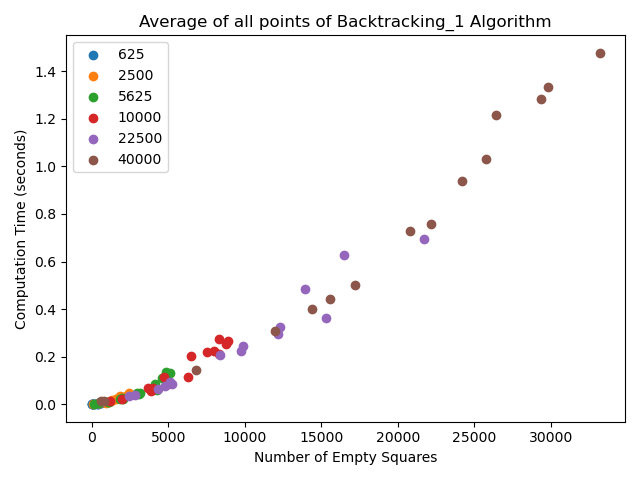
\includegraphics[scale=0.5]{scatter_avg_Backtracking_1-1.png}
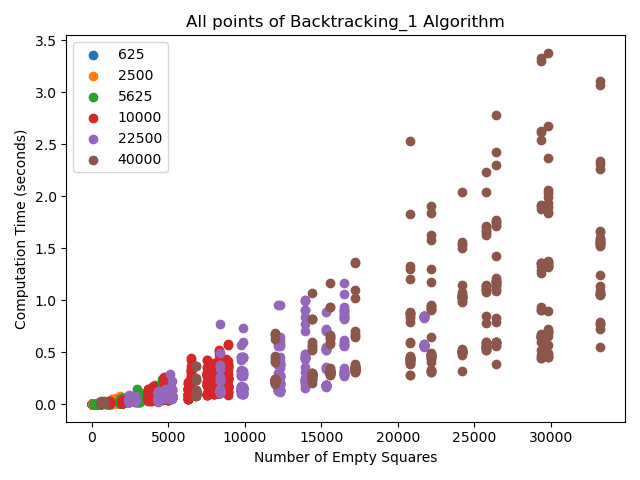
\includegraphics[scale=0.5]{scatter_Backtracking_1-1.png}

\bigskip

\noindent \textit{Backtracking with Heuristic} \\ \\
% Change the images
\includegraphics[scale=0.5]{scatter_avg_Backtracking_w_Heuristic-1.png}
\includegraphics[scale=0.5]{scatter_Backtracking_w_Heuristic-1.png}


From the images it is clear to see that there is a significant difference in
time complexity between the backtracking algorithm and the forward-checking 
with heuristic algorithm. The graph with the average of the points of the
backtracking shows what we believe to be O($n^2$) for time complexity. As the
number of missing cells increases there appears to be an exponential growth
with respect to time. However, in the case of the backtracking algorithm with
a heuristic, it is much more difficult to determine Big-Oh complexity. In this 
specific test case it appears to loosely conform to O(logn) complexity. However,
strictly looking at the y-axis on both of the graphs we can see that the backtracking 
with heuristic algorithm performs much quicker than the previous backtracking algorithm.

\bigskip

Here are some additional examples with some other test cases.

\noindent \textit{Backtracking} \\ \\
% Change the images
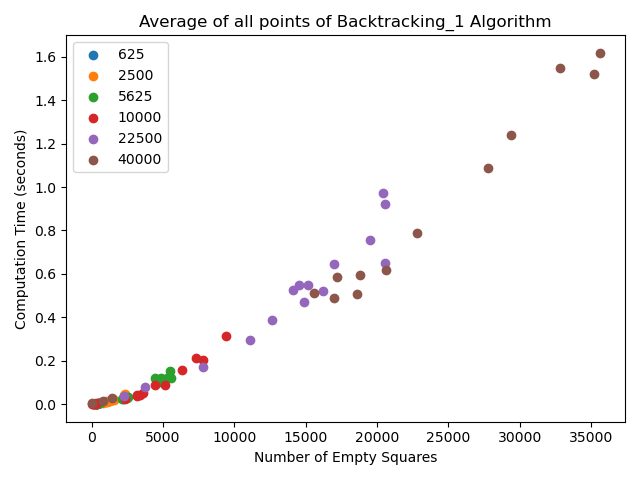
\includegraphics[scale=0.5]{scatter_avg_Backtracking_1-2.png}
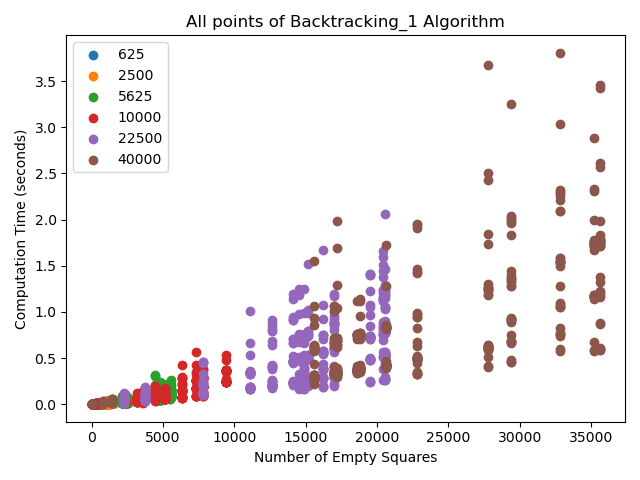
\includegraphics[scale=0.5]{scatter_Backtracking_1-2.png}

\bigskip

\noindent \textit{Backtracking with Heuristic} \\ \\
% Change the images
\includegraphics[scale=0.5]{scatter_avg_Backtracking_w_Heuristic-2.png}
\includegraphics[scale=0.5]{scatter_Backtracking_w_Heuristic-2.png}

Again, with this test case the backtracking algorithm appears to be in the shape of O($n^2$).
However, the backtracking algorithm with heuristic appears to be more in the shape of constant
time, besides the single point which is clearly an outliar. Despite the drastic change in the 
shape of the graph for the backtracking with heuristic algorithm, the backtracking with heuristic algorithm
performs much quicker than the backtracking algorithm that was originally implemented.

\bigskip

\noindent \textit{Backtracking} \\ \\
% Change the images
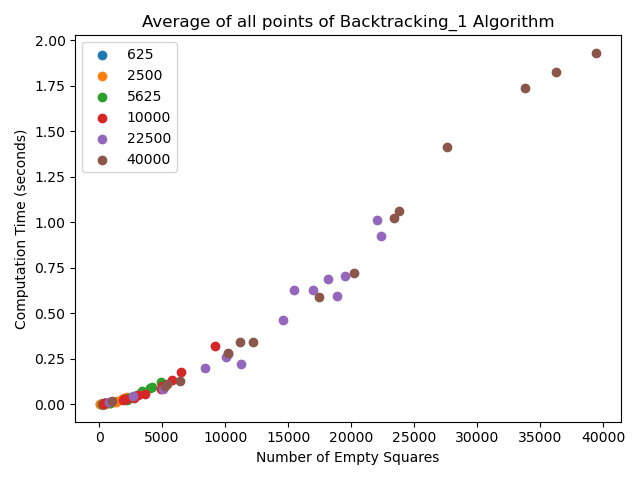
\includegraphics[scale=0.5]{scatter_avg_Backtracking_1-3.png}
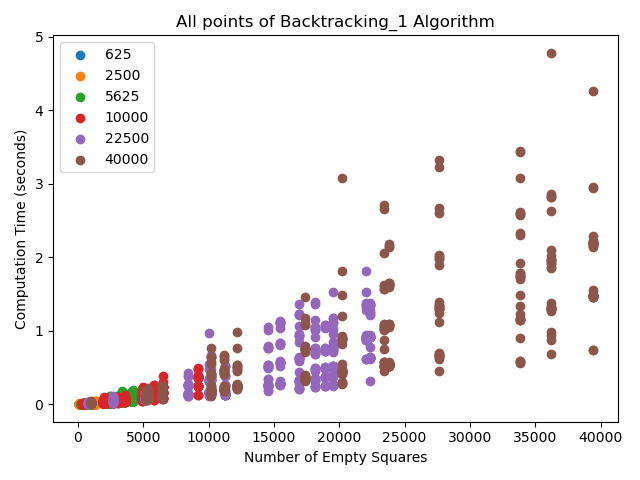
\includegraphics[scale=0.5]{scatter_Backtracking_1-3.png}

\bigskip

\noindent \textit{Backtracking with Heuristic} \\ \\
% Change the images
\includegraphics[scale=0.5]{scatter_avg_Backtracking_w_Heuristic-3.png}
\includegraphics[scale=0.5]{scatter_Backtracking_w_Heuristic-3.png}

These test cases aligned more with the first test case listed above. The
backtracking algorithm again having more of a O($n^2$) complexity while the
backtracking with heuristic algorithm had more of a O(logn) shape. Again, 
the averages of the tests showed that the backtracking algorithm with heuristic
signigicantly outperformed the backtracking algorihtm that was originally used.

\bigskip

Overall, throughout all of the test cases that we ran on both of the algorithms. 
The newly implemented, backtracking with heuristic, significantly outperformed 
our algorithm from the first milestone submission. Solving the problem in the 
fraction of the time. The backtracking algorithm would usually take more than a second
to solve the larger n x m problems while the backtracking with heuristic was capable of
solving it in less than 0.0002 seconds. We are very pleased and surprised with the outcome
of these results. It was very interesting to see such a drastic increase in performance 
when comparing the two algorithms and their ability to solve such large test cases. The largest
test case is a matrix of 40000 cells and our backtracking with heuristic algorithm was capable
of solving it in less than 0.0002 seconds.


% \pagebreak

% \textbf{Summary of the intermediate submission:}

% \bigskip

% \noindent For this assignment, my partner and I used the backtracking algorithm in order
% to solve for the problem. Our program reads in a text file that conatins the 
% number of rows and columns as well as a list of the values that the matrix will
% be made up of. The values will be read in by row,

% \[R_{00},R_{01},R_{02},R_{03},R_{10},R_{11},R_{12},R_{13},R_{20},R_{21},R_{22},R_{23},R_{30},R_{31},R_{32},R_{33}\]

% \noindent The values are then placed in their repsective places in the n $\times$ n matrix.
% The initial empty spaces hold a value of 0, the algorithm will search for the 0's 
% in the matrix and replace them with their correct value. We chose to use a backtracking
% algorithm in order to solve this problem. The psuedo-code for our solution is posted above.
% The solution that we came to is our original code.

\end{document}